\ifx\allfiles\undefined
\documentclass[12pt, a4paper, oneside, UTF8]{ctexbook} 
% ========== 基本包加载 ==========
% 1. 基础宏包
\usepackage{geometry}
\usepackage{fontspec}
\usepackage{amsmath, amsthm, amssymb}
\usepackage{mathrsfs}
\usepackage{enumitem}
\usepackage{graphicx}
\usepackage{array}
\usepackage{ulem}
\usepackage{caption}
\usepackage{tocloft}
% 2. 图形和颜色宏包
\usepackage[dvipsnames]{xcolor}
\usepackage{tikz}
\usetikzlibrary{shapes.geometric}
\usepackage[most]{tcolorbox}
\tcbuselibrary{theorems}
% 3. 页眉页脚宏包
\usepackage{fancyhdr}
\usepackage{lastpage}
% 4. 超链接和书签
\usepackage{hyperref}
\usepackage{bookmark}
% 5. 智能引用
\usepackage{cleveref}
% ========================
% 1. 页面布局设置(窄边距)
\geometry{
  a4paper,
  top=15mm,
  bottom=10mm,
  left=15mm,
  right=15mm,
  headheight=25pt,
  headsep=8mm,
  footskip=15mm,
  includehead,
  includefoot
}
% 2. 字体设置(修改部分)
% 设置全局英文字体
\setmainfont{Times New Roman}
\setsansfont{Arial}
\setmonofont{Consolas}
% 定义字体命令(保持不变)
\newcommand{\kt}{\kaishu} % 楷体
\newcommand{\st}{\songti} % 宋体

\newcounter{theoremcounter}[section]
% 定理环境
\newtcbtheorem[use counter=theoremcounter,number within=section]{theorem}{定理}{
  enhanced,  
  colback=SeaGreen!10!CornflowerBlue!10,
  colframe=RoyalPurple!55!Aquamarine!100!,
  before upper={\parindent 2em}, % 首行缩进
  arc=3pt, % 圆角
  boxrule=1pt, % 边框粗细
}{thm}

% 引理环境
\newtcbtheorem[use counter=theoremcounter,number within=section]{lemma}{引理}{
  enhanced,
  colback=Salmon!20,
  colframe=Salmon!90!Black,
  before upper={\parindent 2em},
  arc=3pt,
  boxrule=1pt,
}{lem}
% 定义环境
\newtcbtheorem[number within=section,number within=section]{definition}{定义}{
  enhanced,
  colback=OliveGreen!10,
  colframe=Green!70,
  before upper={\parindent 2em},
  arc=3pt,
  boxrule=1pt,
}{def}

% 例题和解共享计数器
\newcounter{examplecounter}[section]
% 例题环境
\newtcbtheorem[use counter=examplecounter,number within=section]{example}{例题}{
  enhanced,
  colback=green!5,
  colframe=green!35!black,
  before upper={\parindent 2em},
  arc=5pt,
  boxrule=1pt,
}{ex}
% 结论环境(宋体)
\newtcbtheorem[number within=section]{conclusion}{结论}{
  enhanced,
  colback=Emerald!10,
  colframe=cyan!40!black,
  before upper={\parindent 2em},
  arc=3pt,
  boxrule=1pt,
}{con}
\newtcbtheorem[number within=section]{property}{性质}{
  enhanced,
  colback=Peach!15,              % 浅橙色背景(比纯Orange更柔和)
  colframe=Orange!80!black,  % 深橙色边框带黑色加深
  before upper={\parindent 2em},
  arc=3pt,
  boxrule=1pt,        % 标题加粗与其他环境统一
}{prop}
\newtcbtheorem[number within=section]{criterion}{准则}{
  enhanced,
  colback=Thistle!15,            % 浅紫色背景(柔和)
  colframe=MediumPurple!80!black, % 深紫色边框带黑色加深
  before upper={\parindent 2em},
  arc=3pt,
  boxrule=1pt,
}{crit}
\newtcbtheorem[use counter=theoremcounter,number within=section]{corollary}{推论}{
  enhanced,
  colback=Gold!10,               % 浅金色背景
  colframe=Goldenrod!80!black,   % 深金色边框带黑色加深
  before upper={\parindent 2em},
  arc=3pt,
  boxrule=1pt,        % 标题加粗与其他环境统一
}{cor}
% 传统样式环境(无背景色)
\newtheoremstyle{plain-chinese}% 名称
  {6pt}% 上方空白
  {6pt}% 下方空白
  {\st}% 正文字体(宋体)
  {}% 缩进
  {\heiti}% 标题字体(黑体加粗)
  {.}% 标题后标点
  { }% 标题后空白
  {}% 标题说明
\theoremstyle{plain-chinese}
\newtheorem{solution}{解}[section] % 使用与例题相同的计数器
\newtheorem{remark}{注}[section]
\newtheorem{myproof}{证明}[section]
% 4. 智能引用设置(保持不变)
% ========================
\crefname{theorem}{定理}{定理}
\crefname{lemma}{引理}{引理}
\crefname{definition}{定义}{定义}
\crefname{example}{例题}{例题}
\crefname{conclusion}{结论}{结论}
\crefname{solution}{解}{解}
\crefname{remark}{注}{注}
\crefname{property}{性质}{性质}
\crefname{criterion}{准则}{准则}
\crefname{myproof}{证明}{证明}

% 5. 数学字体设置(修改)
\usepackage{unicode-math} % 更好的数学字体支持
\setmathfont{Latin Modern Math} % 使用默认数学字体
% ========== 自定义命令(保持不变) ==========
\newcommand{\R}{\mathbb{R}} % 实数集
\newcommand{\C}{\mathbb{C}} % 复数集
\newcommand{\Z}{\mathbb{Z}} % 整数集
\newcommand{\N}{\mathbb{N}} % 自然数集
\newcommand{\dif}{\mathrm{d}} % 微分符号

% ========== 图形路径设置(保持不变) ==========
\graphicspath{{./flg/}} % 图片路径

% 6. 页眉页脚设置
% ========================
\usepackage{fancyhdr}
\usepackage{lastpage} % 获取总页数
\pagestyle{fancy}
\fancyhf{} % 清除所有页眉页脚设置

% 通用设置
\fancyhead[L]{\small\kt 高中数学~解析几何} % 左边:书名(楷体)
\fancyhead[C]{\small\st 居敬持志~守正出奇}
\fancyhead[R]{\small\st 还在尬黑出品} % 中间:声明(宋体)
\fancyfoot[C]{\thepage} % 居中页码(自定义样式)

% 正文部分设置
\fancyhead[R]{\small\st\rightmark} % 右边:章节名称(宋体)

% 前言部分设置(使用罗马数字页码)
\fancypagestyle{frontmatter}{
    \fancyhf{}
    \fancyhead[L]{\small\kt 高中数学~解析几何}
    \fancyhead[C]{\small\st 前言}
    \fancyhead[R]{还在尬黑出品} % 前言部分无章节名称
    \fancyfoot[C]{\thepage}
    \renewcommand{\headrulewidth}{0.4pt} % 页眉线
    \renewcommand{\footrulewidth}{0pt} % 无页脚线
    \pagenumbering{Roman} % 罗马数字页码
}

% 目录部分设置(使用罗马数字页码,延续前言页码)          % 去掉标题下方的横线
\fancypagestyle{tocmatter}{
    \fancyhf{}
    \fancyhead[L]{\small\kt 高中数学~解析几何}
    \fancyhead[C]{\small\st 目录} % 居中显示"目录"
    \fancyhead[R]{\small\st 还在尬黑出品} 
    \fancyfoot[C]{\thepage}
    \renewcommand{\headrulewidth}{0.4pt}
    \renewcommand{\footrulewidth}{0pt}
    % 注意:这里不重置页码,延续前面的罗马数字
}
% 正文部分设置(使用阿拉伯数字页码)
\fancypagestyle{mainmatter}{
    \fancyhf{}
    \fancyhead[L]{\small\kt 高中数学~解析几何}
    \fancyhead[C]{\small\st 居敬持志~~守正出奇}
    \fancyhead[R]{\small\st\rightmark}
    \fancyfoot[C]{\thepage}
    \renewcommand{\headrulewidth}{0.4pt} % 页眉线
    \renewcommand{\footrulewidth}{0pt} % 无页脚线
    \pagenumbering{arabic} % 阿拉伯数字页码
}
% 设置章节标记格式
\renewcommand{\chaptermark}[1]{\markboth{#1}{}}
\renewcommand{\sectionmark}[1]{\markright{\thesection.\ #1}}

% 8. 章节标题字体设置
\ctexset{
    chapter = {
        format = \centering, % 整体居中
        nameformat = \kaishu\LARGE, % 编号部分黑体加粗
        titleformat = \songti\LARGE, % 标题部分宋体
        aftername = \quad, % 编号和标题之间的间距
        beforeskip = 30pt, % 标题前的垂直间距
        afterskip = 20pt, % 标题后的垂直间距
        name = {第,章}, % 中文章节编号格式
        number = \chinese{chapter}, % 使用中文数字
    },
    section = {
        format = \raggedright, % 左对齐
        nameformat = \heiti\large, % 编号部分黑体加粗
        titleformat = \songti\large, % 标题部分宋体
        aftername = \quad, % 编号和标题之间的间距
        beforeskip = 15pt, % 标题前的垂直间距
        afterskip = 6pt, % 标题后的垂直间距
    },
    subsection = {
        format = \raggedright, % 左对齐
        nameformat = \heiti\normalsize, % 编号部分黑体加粗
        titleformat = \songti\normalsize, % 标题部分宋体
        aftername = \quad, % 编号和标题之间的间距
        beforeskip = 6pt, % 标题前的垂直间距
        afterskip = 3pt, % 标题后的垂直间距
    }
}
\begin{document}
% \begin{titlepage}
    \centering
    % 顶部留白
    \vspace*{0.5cm}
    
    {\fontsize{80}{80}\selectfont\songti 高中数学 \par}
    \vspace{0.1cm} % 减少间距
    
    % 副标题
    {\fontsize{65}{65}\selectfont\songti 解析几何讲义 \par}
    \vspace{1cm} % 减少间距
    
    % 作者信息
    {\Large \kaishu{作者:} 还在尬黑 \par}
    \vspace{0.1cm}
    
    % 版本信息
    {\Large \kaishu{版本:} 第1版 \par}
    \vspace{0.1cm}
    
    % 日期
    {\Large \kaishu{日期:} \today \par}
    \vspace{0.1cm}
    
    % 添加图片
    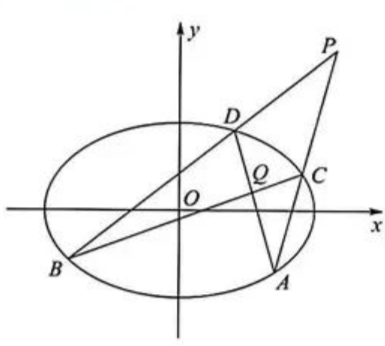
\includegraphics[width=0.5\textwidth]{flg/example.png} % 调整图片大小
    \par\vspace{1cm}
    {\small \copyright{} 2025 版权所有}
\end{titlepage}
\else
\fi

\chapter{演示}
\section{导数的概念}

\begin{defn}
    设函数$y=f(x)$在点$x_0$的某个邻域内有定义,当自变量$x$在$x_0$处取得增量$\Delta{x}$(点$x_0+\Delta{x}$在该邻域内),因变量取得增量
    \[ \Delta{y}=f(x_0+\Delta{x})-f(x_0) \]
    如果$\Delta{y}$与$\Delta{x}$之比当$\Delta{x}\to 0$时的极限存在,那么称函数$y=f(x)$在点$x_0$处可导,并称这个极限为函数$y=f(x)$在$x_0$处的导数,记为$f'(x)$,即
    \[
        f'(x) = \lim_{\Delta{x}\to0}\frac{\Delta{y}}{\Delta{x}} = \lim_{\Delta{x}\to 0}\frac{f(x_0+\Delta{x})-f(x_0)}{\Delta{x}}
    \]
    或记为$y'|_{x=x_0},\;\dfrac{\d y}{\d x}\Big|_{x = x_0},\;\dfrac{\d f(x)}{\d x}\Big|_{x=x_0},\;f'(x) = \lim\limits_{x\to x_0}\dfrac{f(x)-f(x_0)}{x-x_0}$.
\end{defn}

\begin{lemma}[瞎编的引理]
    好好学习 => 天天向上
\end{lemma}

\begin{thm}[瞎编的定理]
    山不让尘,川不辞盈
\end{thm}

\begin{corollary}[瞎编的推论]
    你小子没点赞.
\end{corollary}

\begin{criterion}[夹逼准则]
    $a(x) < b(x) < c(x)$,且$\lim{a} = \lim{c} = A$,那么$\lim{b} = A$
\end{criterion}

\begin{proposition}
    差若毫厘,谬以千里.
\end{proposition}

\begin{example}
    求 $ 1+2 = ?$
\end{example}

\begin{solution}
    $\displaystyle 1 + 2 = (1+2)\int_0^1 x^2 \d x + (1+2)\int_0^1 x^2 \d x + (1+2)\int_0^1 x^2 \d x$
\end{solution}

\begin{rmk}
    我不会
\end{rmk}

\begin{proof}
    $1 + 2 = 2 + 1$.
\end{proof}

\section{偏导数}
\subsection{偏导数的定义及其计算法}
\begin{defn}
    设函数$z=f(x,\,y)$在点$(x_0,\,y_0)$的某一邻域内有定义,当$y$固定在$y_0$而$x$在$x_0$处有增量$\Delta x$时,相应的函数有增量$f(x_0 + \Delta{x},\,y_0) - f(x_0,\,y_0)$,如果
    \[
        \lim_{\Delta{x} \to 0}\frac{f(x_0 + \Delta{x},\,y_0)-f(x_0,\,y_0)}{\Delta{x}}
    \]
    存在,那么称此极限为函数$z=f(x,\,y)$在点$(x_0,\,y_0)$处对$x$的偏导数(一点处的偏导),记作:
    \[
        \frac{\partial z}{\partial x}\Big| _{x=x_0,\, y=y_0} ,\enspace \frac{\partial f}{\partial x}\Big| _{x=x_0,\, y=y_0} ,\enspace f_x(x_0,y_0),\enskip {f_x}'(x_0,y_0)
    \]
    类似地,函数$z=f(x,\,y)$在点$(x_0,\,y_0)$处对$y$的偏导数定义为
    \[
        \lim_{\Delta{y} \to 0}\frac{f(x_0,\,y_0+\Delta{y})-f(x_0,\,y_0)}{\Delta{y}}
    \]
    记作同上,定义可推广到$n$元函数.
\end{defn}

\begin{example}
    求$z = x^2\sin{2y}$的偏导数.
\end{example}
\begin{solution}
    易得$\dfrac{\partial{z}}{\partial{x}} = 2x\sin{2y}+x^2(\sin{2y})' = 2x\sin{2y}$,$\dfrac{\partial{z}}{\partial{y}} = 2x^2\cos{2y}$.
\end{solution}

\myspace{1}

\begin{center}
    {\LARGE 你小子记得点赞!}
\end{center}

\ifx\allfiles\undefined
\end{document}
\fi